\documentclass[lettersize,journal]{IEEEtran}
\usepackage{amsmath,amsfonts}
\usepackage{algorithmic}
\usepackage{algorithm}
\usepackage{array}
\usepackage[caption=false,font=normalsize,labelfont=sf,textfont=sf]{subfig}
\usepackage{textcomp}
\usepackage{stfloats}
\usepackage{url}
\usepackage{verbatim}
\usepackage{graphicx}
\usepackage{cite}
\usepackage{multirow}
\usepackage{booktabs}
\usepackage{xcolor}
\usepackage{tabularx}

\hyphenation{op-tical net-works semi-conduc-tor IEEE-Xplore}
\input macro
% updated with editorial comments 8/9/2021

\begin{document}

\title{Shaping a Smarter Electromagnetic Landscape: \\An Overview of IAB, NCR, and RIS in\\ 5G Standardization and Beyond}

\author{Chao-Kai~Wen,~\IEEEmembership{Senior Member,~IEEE},~Lung-Sheng~Tsai,~Arman~Shojaeifard,~\IEEEmembership{Senior~Member,~IEEE}, Pei-Kai~Liao,~Kai-Kit~Wong,~\IEEEmembership{Fellow,~IEEE},~and~Chan-Byoung~Chae,~\IEEEmembership{Fellow,~IEEE}

\thanks{{C.-K.~Wen} is with the Institute of Communications Engineering, National Sun Yat-sen University, Kaohsiung 80424, Taiwan, Email: {\rm chaokai.wen@mail.nsysu.edu.tw}.}
\thanks{{L.-S.~Tsai} and {P.-K.~Liao} are with the MediaTek Inc., Hsinchu, Taiwan, Email: {\rm Longson.Tsai@mediatek.com, pk.liao@mediatek.com}.}
\thanks{{A.~Shojaeifard} is with InterDigital, London EC2A 3QR, U.K., Email: {\rm Arman.Shojaeifard@InterDigital.com}.}
\thanks{{K.-K.~Wong} is with Department of Electronic and Electrical Engineering, University College London, UK, Email: {\rm kai-kit.wong@ucl.ac.uk}. He is also affiliated with Yonsei Frontier Lab., Yonsei University, Korea.}
\thanks{{C.-B.~Chae} is with Yonsei University, Seoul 03722, Korea, Email: {\rm cbchae@yonsei.ac.kr}.}
}

% The paper headers
%\markboth{IEEE Communications Standards Magazine}%
%{Shell \MakeLowercase{\textit{et al.}}: A Sample Article Using IEEEtran.cls for IEEE Journals}

%\IEEEpubid{0000--0000/00\$00.00~\copyright~2021 IEEE}
%% Remember, if you use this you must call \IEEEpubidadjcol in the second
%% column for its text to clear the IEEEpubid mark.

\maketitle


\begin{abstract}

The main objective of 5G and beyond networks is to provide an optimal user experience in terms of throughput and reliability, irrespective of location and time. To achieve this, traditional fixed macro base station deployments are being replaced by more innovative and flexible solutions, such as wireless backhaul and relays. This article focuses on the evolution and standardization of these advancements, which are shaping the electromagnetic (EM) landscape. Specifically, we explore Integrated Access and Backhaul (IAB) nodes, offering a cost-efficient and agile alternative to fiber backhaul. We  also discuss Network-Controlled Repeaters (NCRs) and the emergence of Reconfigurable Intelligent Surfaces (RIS) actively adapting the wireless environment. The article provides an overview of the 5G features and ongoing developments in 3GPP Release 18 related to these intelligent EM entities, highlighting the expected evolution of future wireless networks in terms of architecture, operations, and control signals.
\end{abstract}

%\begin{IEEEkeywords}
% IAB, NCR, Reconfigurable Intelligent Surfaces.
%\end{IEEEkeywords}

\begin{figure*}[b]
\centering
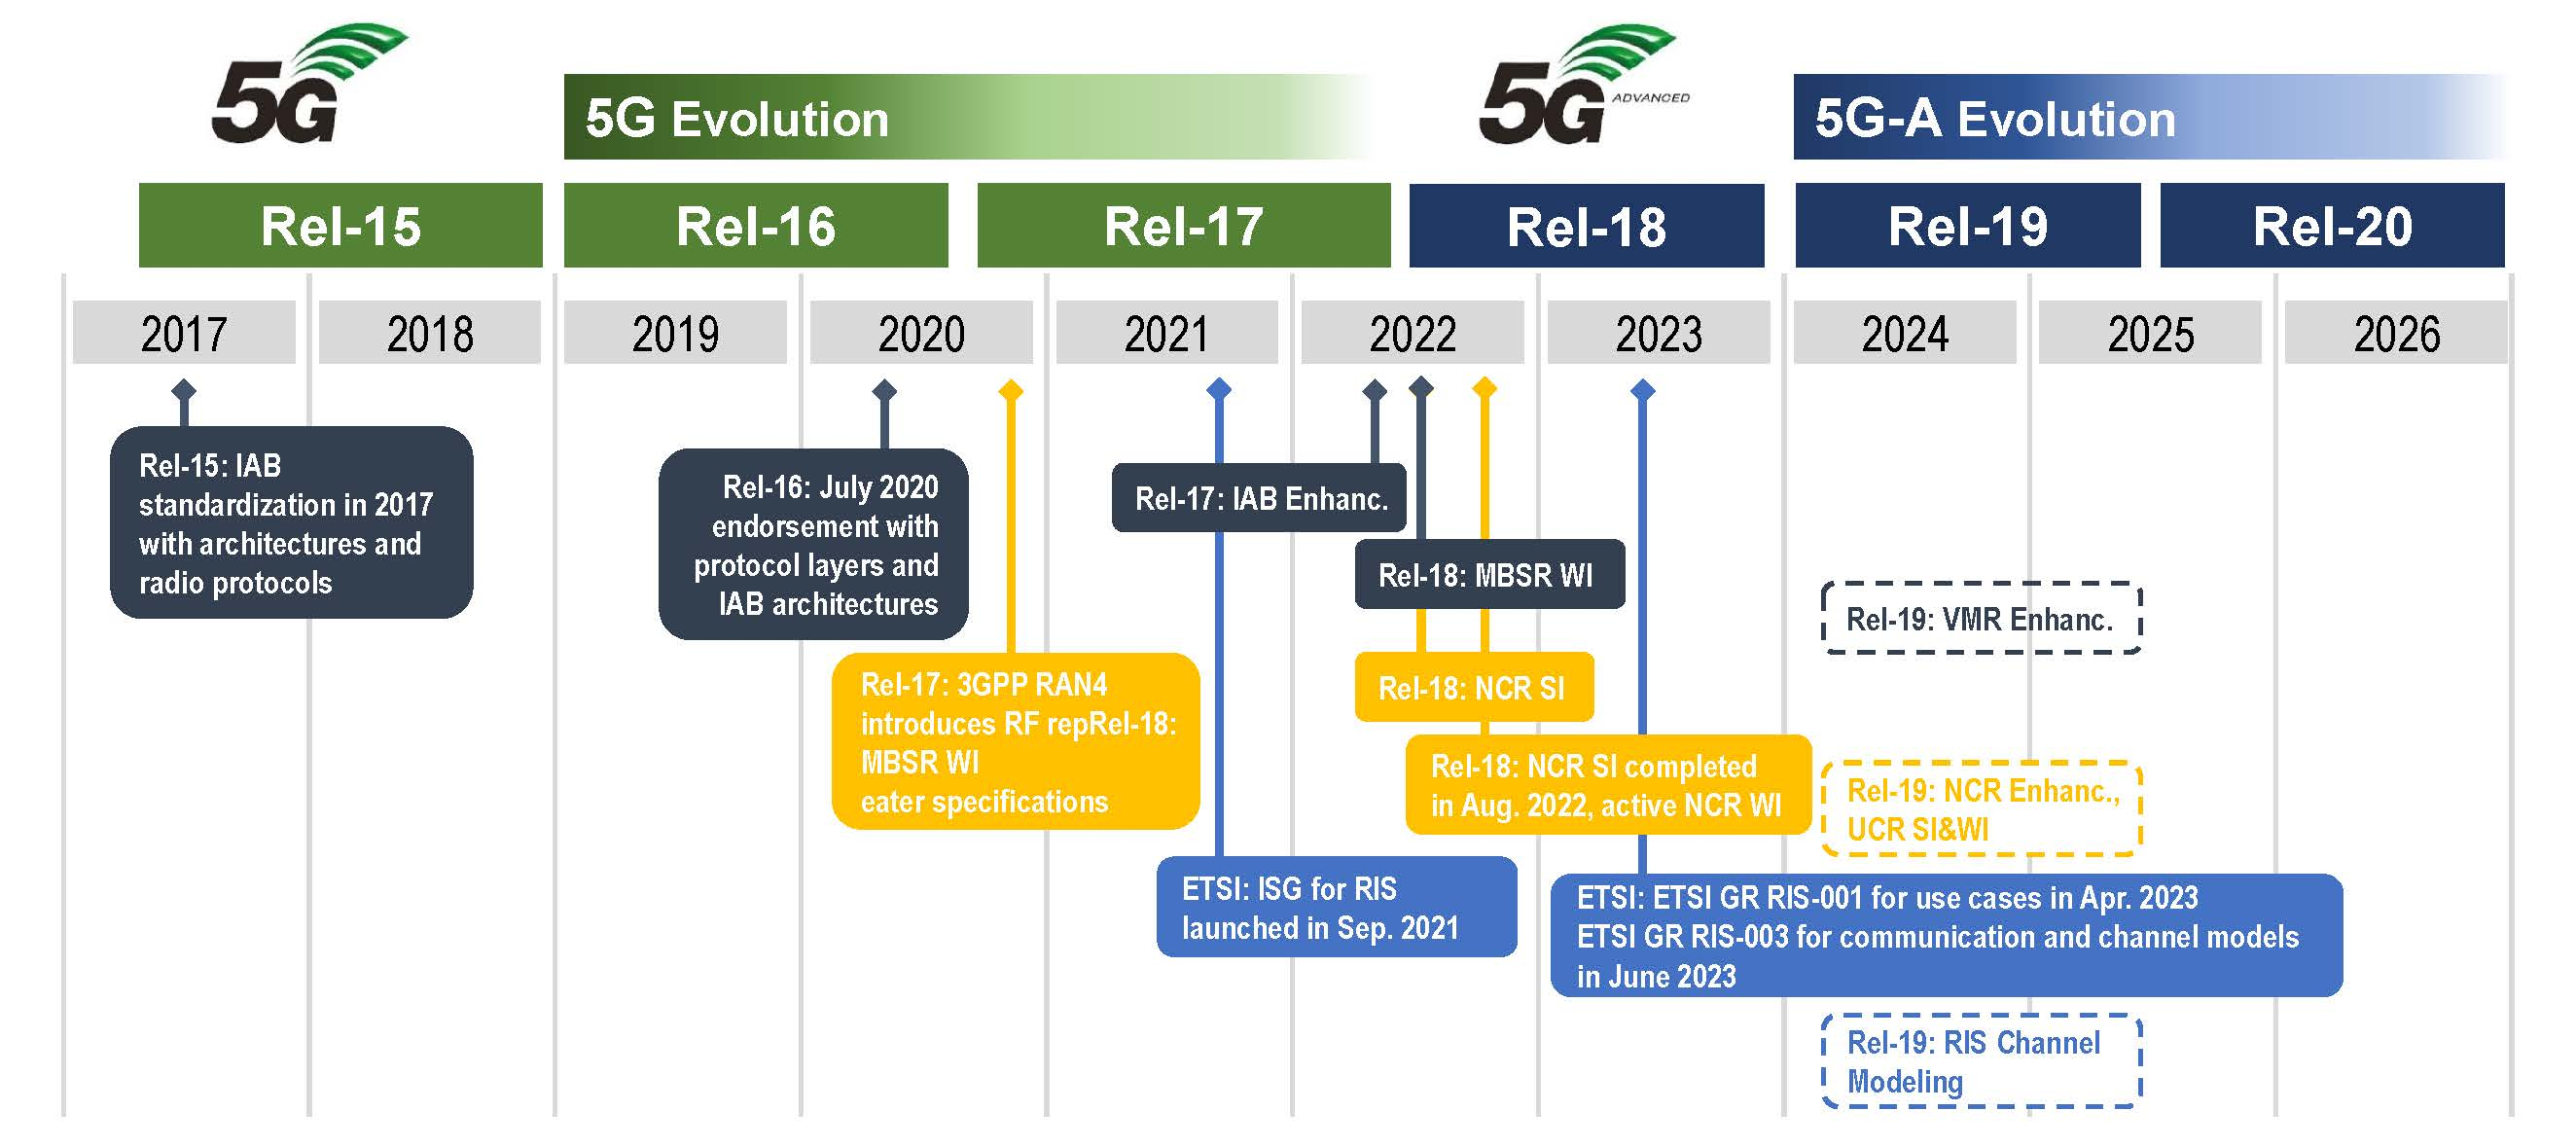
\includegraphics[width=6.0in]{Figs/3GPP_Roadmap.jpg}
\caption{5G standardization for IAB, NCR, and RIS.}
\label{fig:3GPP_Roadmap}
\end{figure*}


\section{Introduction}

\IEEEPARstart{T}{he} primary goal for 5G and beyond wireless networks is to satisfy user experience requirements for throughput and reliability, while simultaneously maintaining energy efficiency across all locations. Cellular networks traditionally relied on fixed macro base stations (BSs) for deployment. However, this approach may not offer sufficient coverage in densely populated urban areas or at higher frequencies. Network densification can address these coverage gaps, but creating new infrastructure from scratch is time-consuming and poses significant challenges due to cost, power sourcing, real estate permissions, regulatory approvals, and backhaul availability. In this context, wireless backhaul emerges as a feasible solution for enabling flexible and dense network deployments.

Wireless backhaul has been extensively studied, with the LTE relay playing a role in standardization efforts during LTE Release 10 \cite{3GPP-Rel10}. However, due to the limited performance boost and the complexity of relay features, few operators adopted LTE relay. With the rise of dense 5G new radio (NR) networks and advancements in beamforming technology, there is renewed interest in developing an integrated access and backhaul (IAB) solution. This solution offers a faster and more cost-efficient alternative to fiber backhaul. Figure \ref{fig:3GPP_Roadmap} depicts the 3GPP's IAB roadmap from 5G to 5G Advanced. Studies on IAB architectures and radio protocols began with a study item (SI) within 3GPP Release 15. In Release 16, a multi-hop NR-based IAB solution was officially introduced, with the objective of using the existing 5G radio air interface for wireless backhaul and meeting specified electromagnetic (EM) compatibility requirements. Standardization efforts continued in Release 17, with a focus on enhancing IAB network performance through topology adaptation, duplexing, and efficiency enhancements. Additionally, Release 18 introduced a work item (WI) to explore architectural and system-level enhancements for 5G networks with mobile BS relays mounted on vehicles, termed Vehicle Mounted Relay (VMR) \cite{TR-23.700}.

Apart from IAB, employing non-regenerative RF repeaters is a simpler solution for improving network coverage. RF repeaters, utilizing the amplify-and-forward operation, have been widely deployed in commercial 2G, 3G, and 4G networks. As 5G NR technology migrates to higher frequencies, signal propagation conditions may deteriorate, necessitating the critical implementation of RF repeaters. To accommodate this increasing demand, 3GPP RAN4 introduced specifications for RF repeaters in Release 17 \cite{RP-202813}. These specifications lay out the RF and Electromagnetic Compatibility requirements for FR1 and FR2, ensuring compatibility in typical commercial environments.

Although RF repeaters are cost-effective for expanding network coverage, they are limited in terms of accommodating factors that enhance network performance and efficiency, such as dynamic DL/UL configurations, adaptive spatial beamforming, and ON-OFF stages. To circumvent these limitations, 3GPP initiated a new SI in May 2022 focusing on network-controlled repeaters (NCRs). NCRs inherit the amplify-and-forward operation of RF repeaters but also receive control information from the 5G gNB to function more efficiently. With this control information, NCRs enable transmissions and receptions with improved spatial directivity, facilitate network integration, and minimize unnecessary interference. The SI was finalized in August 2022, and 3GPP is currently developing the NCR WI \cite{RP-222673}. Figure~\ref{fig:3GPP_Roadmap} provides an overview of 3GPP's NCR roadmap.

Reconfigurable Intelligent Surfaces (RIS) are an emerging technology that leverages reconfigurable surface technology to adapt to the propagation environment. Primarily using passive components and eliminating the need for expensive active components like power amplifiers, RIS provides benefits such as lower hardware costs, reduced energy consumption, and versatile deployment options on various structures like walls, buildings, and lamp posts. Compared to IAB and NCR, RIS stands out due to its cost-effectiveness and adaptability.

As for standardization, RIS has not yet been studied in 3GPP. While some companies proposed including RIS as a SI in 3GPP for Release 18, most considered it premature and suggested exploring it for 6G technology instead. Consequently, the proposal was not approved for Release 18. To address standardization, the ETSI Industry Specification Group (ISG) for RIS was established in September 2021. It serves as the pre-standardizing group for RIS, aiming to define use cases, deployment scenarios, and requirements to establish global standardization. The group's objective is to provide a framework for dynamically controlling radio signals between transmitters and receivers, transforming the wireless environment into a service. Recently, ETSI released its first Group Report in April 2023, identifying relevant RIS use cases (ETSI GR RIS-001 \cite{ETSI-GR-RIS-001}), and subsequently, a new Report in June 2023, exploring communication and channel models (ETSI GR RIS-003 \cite{ETSI-GR-RIS-003}). Figure~\ref{fig:3GPP_Roadmap} showcases ETSI's progress on RIS.

With the standardization of IAB, NCR, and RIS, future networks are anticipated to incorporate various wireless nodes to optimize network performance, reduce costs, and minimize power consumption \cite{Flamini-TAP22}. 3GPP is currently entering the second phase of 5G standardization, referred to as 5G-Advanced, building upon the 5G baseline established in 3GPP Releases 15, 16, and 17. The 3GPP Release 19 RAN workshop (Rel-19 WS) was held on June 15-16, 2023, attracting strong global interest with submissions from over 80 different companies/organizations. 3GPP Release 19, expected to start in 2024, may incorporate some enhancements to the IAB and NCR and initiate a study on RIS. RIS shares deployment scenarios with IAB and NCR, and the progression of IAB and NCR within existing 5G and ongoing 5G-Advanced provides mutual reference among them and lays a foundational reference for future RIS standardization. This article aims to provide an overview of 5G NR features pertinent to IAB and NCR, anticipating the evolution of future wireless networks in terms of architecture, operations, and control signals. Furthermore, insights into their evolution and the latest status of RIS based on the ETSI ISG RIS will be provided.

\section{IAB}

\begin{figure*}
\centering
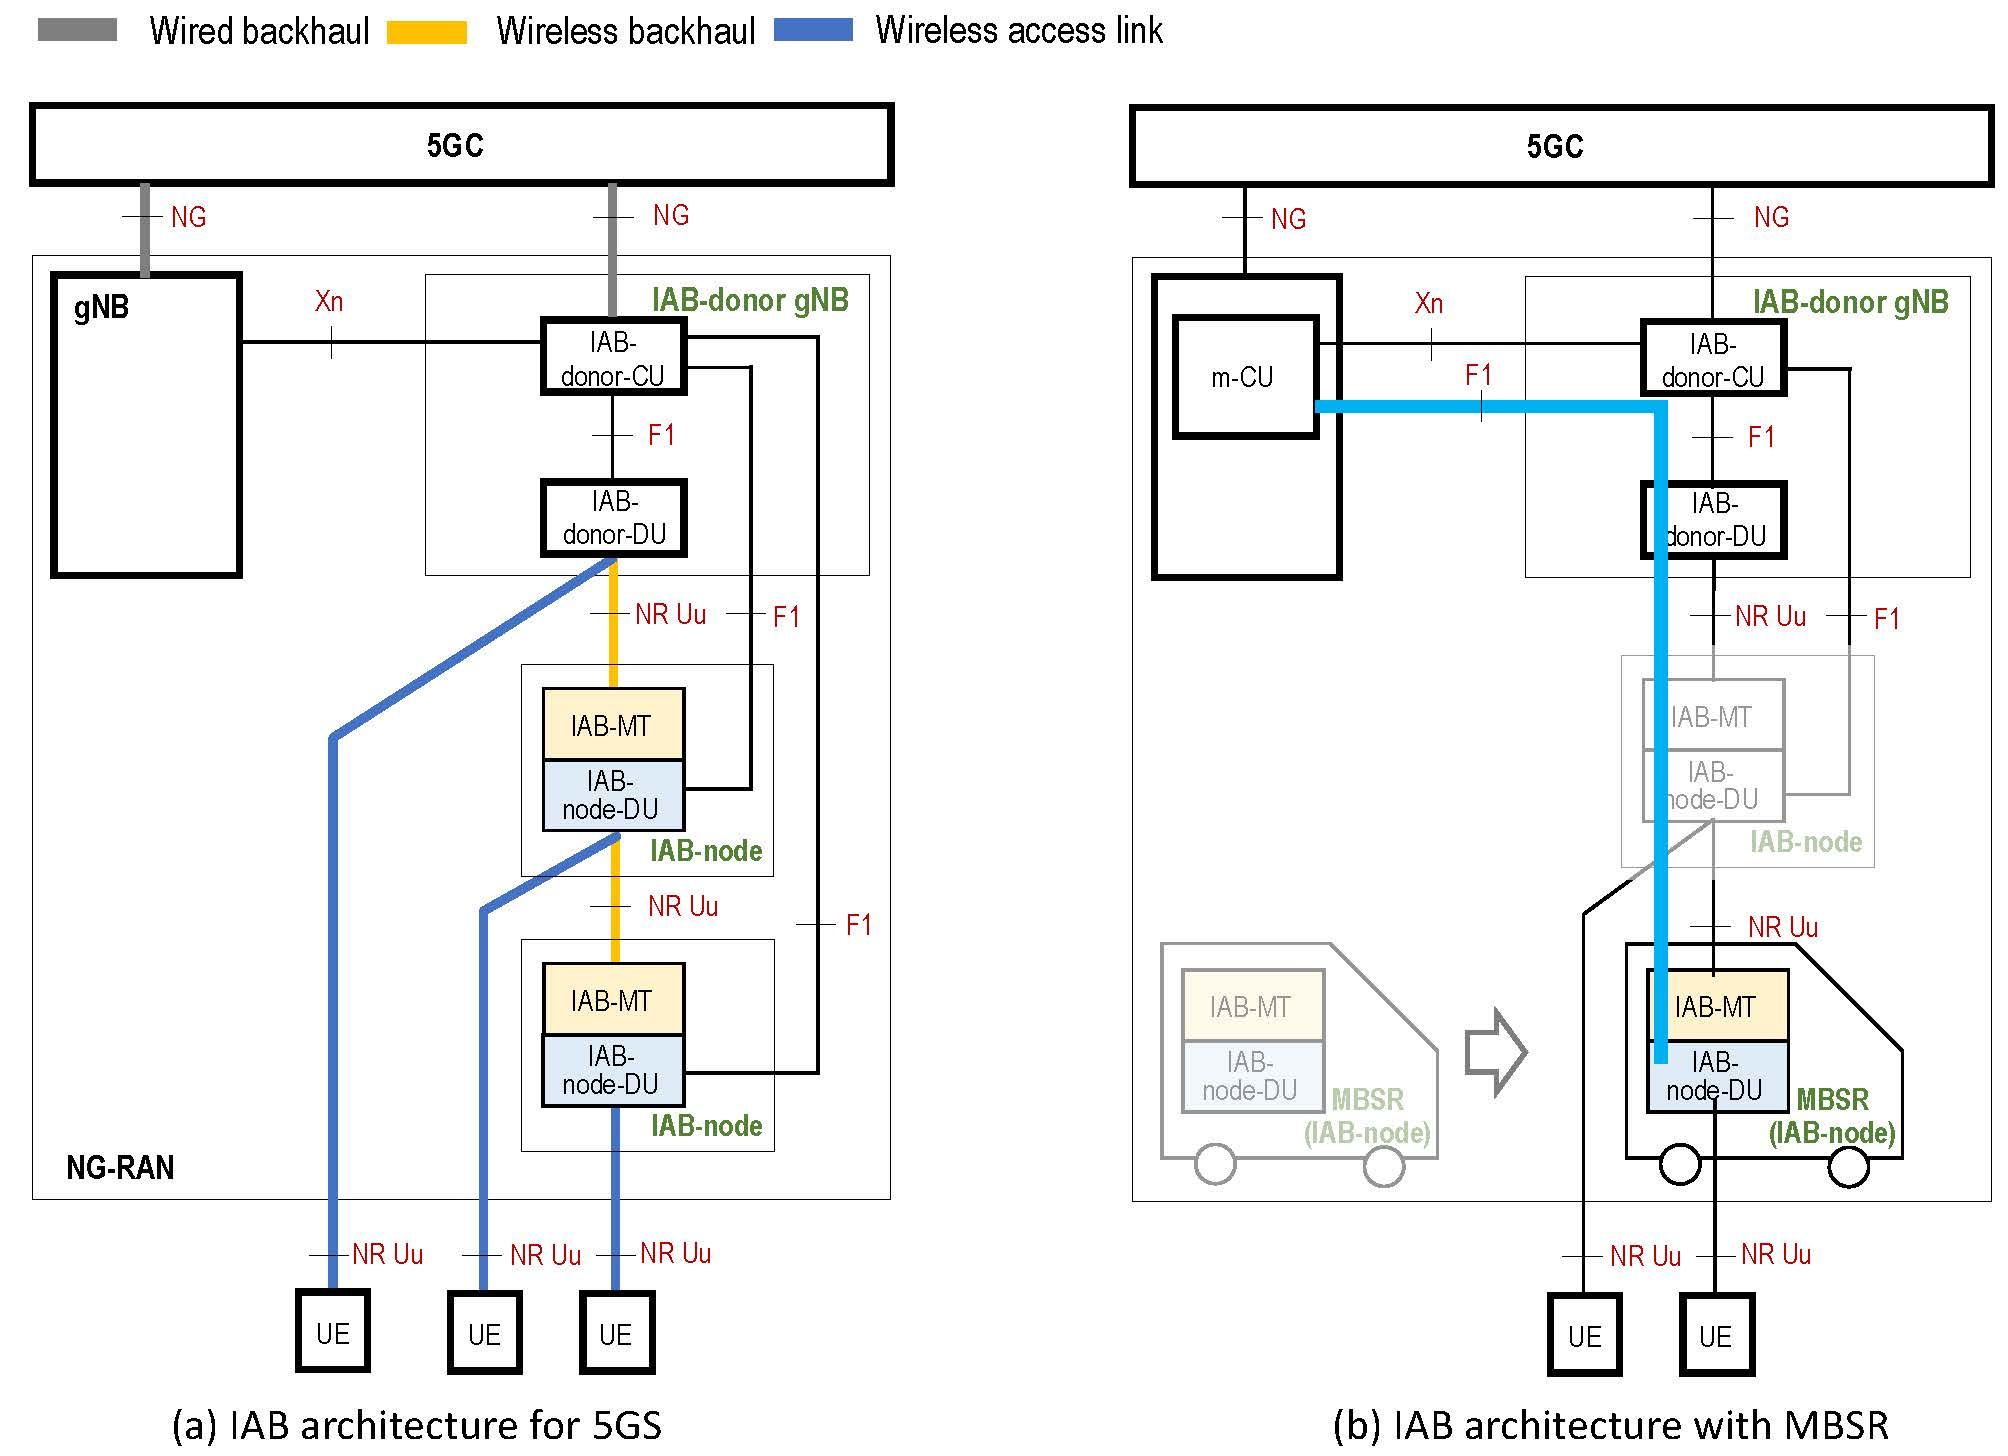
\includegraphics[width=5.5in]{Figs/IAB_architecture.jpg}
\caption{IAB architectures for 5GS and MBSR.}
\label{fig:IAB_architecture}
\end{figure*}

In Release 16, a multi-hop NR-based IAB solution was introduced, aiming to reuse the existing 5G radio air interface for in-band or out-of-band wireless backhaul.
In this section, we explore the architecture of IAB, including its network topology, resource allocation mechanisms, and recent enhancements introduced in Release 18.

\subsection{IAB Architecture}

The architecture of IAB, depicted in Figure \ref{fig:IAB_architecture}(a), defines two types of network nodes \cite{TS-38.300}.

\subsubsection{IAB-donor} The IAB-donor acts as the central control node in the IAB network, composed of an IAB-donor-CU and an IAB-donor-DU connected through a wired F1 interface. The IAB-donor-DU handles the lower protocol layers (PHY, MAC, and RLC), while the IAB-donor-CU oversees the upper protocol layers (PDCP and SDAP/RRC).\footnote{Abbreviations: Physical (PHY), medium access control (MAC), radio link control (RLC), packet data convergence protocol (PDCP), and service data adaptation protocol (SDAP) / radio resource control (RRC).} This division permits time-sensitive functions to be conducted by the IAB-donor-DU, which is closer to the served nodes, and the remaining functions by the IAB-donor-CU, which has superior processing capacity \cite{IAB-Overview22,IAB-chae}.

\subsubsection{IAB-node} The IAB-node is a wireless relay node within the IAB network, tasked with initiating access to the parent node above it and providing access services to child nodes below it. As such, the IAB-node comprises two functional modules: the IAB Mobile Termination (IAB-MT) and the IAB-node-DU. The IAB-MT links an IAB node with the DU of the parent/upstream node, which can either be an IAB-donor or another IAB-node. The IAB-node-DU (or IAB-donor-DU) caters to the UEs and potentially downstream IAB-nodes in instances of multi-hop wireless backhauling.

IAB-nodes function as L2 regenerative relays, decoding and re-encoding each received packet prior to retransmission. This mechanism applies to packets received from the IAB-donor, UEs, or other IAB-nodes.

\subsection{IAB Network Topology}

Figure \ref{fig:IAB_architecture}(a) depicts the topology of an IAB network. The network originates from an IAB-donor, which serves as the central control node and traffic convergence point between the access and core network. The network expands in a tree-like structure through wireless links, connecting multiple intermediate nodes or IAB-nodes. These IAB-nodes provide user equipment (UE) access services and enable multi-hop transmissions, directing backhaul traffic to their respective child or upstream nodes.

The IAB-donor-CU establishes connections with all DU components in the IAB topology using wired and wireless F1 interfaces. It manages traffic to and from the core network while coordinating the operations of the entire IAB topology. For its child IAB-nodes, the IAB-donor provides wireless backhaul links within its radio coverage. From the perspective of UEs, there is no distinction between IAB-nodes, IAB-donors, and regular NR BSs. They all provide access links to UEs within their radio coverage through the IAB-DU module. The IAB-MT module, similar to a UE with a subset of UE functions, enables the IAB-node to connect to its parent DU node through the NR air interface.

During the initial power-up of an IAB-node, it needs to access the IAB network as a UE, acquire an IP address, and establish a wireless F1 interface between the IAB-node-DU and the IAB-donor-CU. Once the IAB-node-DU is configured, it can operate as a relay node within the network topology.

In a single-hop transmission scenario, the UE directly receives network services through the access link provided by the IAB-donor. However, in a multi-hop transmission scenario, the UE accesses the network via a neighboring IAB-node and utilizes the wireless backhaul function for multi-hop transmissions. The uplink transmission is relayed to the IAB-donor through multiple wireless backhaul links before reaching the core network, and the downlink transmission follows the reverse process.


\begin{table}[!t]
\caption{Comparisons of IAB and NCR.}\label{tab:IAB_vs_NCR}
\centering
\begin{tabular}{|l|c|c|}
\hline
 & \textbf{IAB} & \textbf{NCR} \\
\hline
3GPP Stage & Part of Rel-16 & WI in Rel-18 \\
\hline
Backhaul Link & Out-of-band/In-band & In-band \\
\hline
Architecture & Multi-hop & Single-hop \\
\hline
Deployment & Stationary/Mobile & Stationary \\
\hline
Operation & Decode and forward & Amplify and forward \\
\hline
Duplex Mode & Half duplex/FD & FD \\
\hline
UE Transparency & Not transparent & Transparent \\
\hline
Power Saving & Specifics vary & Uses ON-OFF information \\
\hline
\end{tabular}
\end{table}

\subsection{IAB Resource Allocation Mechanism}

The IAB-MT can utilize a standalone or shared IAB-DU antenna, with the shared antenna offering better integration and range. One major challenge in IAB deployment is the potential interference between wireless links, especially when the transceiver antennas designated for the MT and DU functions of an IAB node lack sufficient isolation. To overcome this challenge, various wireless resource allocation mechanisms have been developed to isolate signals in terms of time, frequency, or space, thus mitigating interference and improving the overall network performance of the IAB.

In 3GPP Release 16, the IAB network predominantly employs Time-Division Multiplexing (TDM) as its wireless resource allocation mechanism. The parent node allocates available time resources to the child links of the IAB node, ensuring that the MT and DU sides have non-overlapping receive and transmit states. This allocation effectively eliminates self-interference between parent and child links.

In 3GPP Release~17, additional enhancements are introduced to the IAB techniques, including support for Frequency/Space-Division Multiplexing (FDM/SDM). These mechanisms allow for the application of multiple techniques to further mitigate self-interference. Moreover, Release~17 introduces a Full Duplex (FD) scheme as an advanced feature of the IAB network. This FD scheme utilizes self-interference cancellation algorithms to suppress self-interference below the noise level, enabling all links of an IAB node to transmit and receive over the same time-frequency resources \cite{IAB-chae}. This significant advancement enhances spectrum efficiency and reduces latency within the IAB network.

\subsection{IAB in Release 18 and Outlook}

Wireless backhaul enables the deployment of mobile cells, with Mobile Base Station Relays (MBSRs) often installed in vehicles like buses or trains, known as VMRs, to provide coverage for UE within or near the vehicle. 3GPP Release 18 focuses on architecture enhancements for MBSRs \cite{TR-23.700}. MBSRs operate within a single-hop topology framework, where the lower IAB node aligns with the MBSR, and an intermediate IAB node may exist as long as it does not function as an MBSR, as shown in Figure~\ref{fig:IAB_architecture}(b).

Due to the wide coverage area of an MBSR, it may need to switch its IAB donor, which can cause disruptions to the PDCP and RRC connections of the UEs it serves. To mitigate these disruptions, the introduction of a mobile control unit (m-CU) is proposed. By ensuring that the MBSR's DU is under the service of the m-CU, the MBSR can move across a larger RAN coverage area without requiring a change in the m-CU. This allows the mobility of the MBSR between IAB donors to remain transparent to the UEs connected to it, as long as the control remains within the same m-CU. In Figure \ref{fig:IAB_architecture}(b), the m-CU corresponds to the originating IAB-donor-CU, maintaining the F1 connection with the migrating IAB-node-DU, while the IAB-MT transitions to the target topology. This approach ensures service continuity for UEs without the need for UE handovers.

Release 18 also addresses other pertinent challenges associated with MBSRs, such as implementing location services for UEs accessing the network through mobile or roaming MBSRs, ensuring accurate Cell ID/Tracking Area Code information despite MBSR movements, and developing efficient controls for managing UE access to the 5G network via MBSRs. Geographic constraints and legacy UE support are also factored in. Further enhancements to the MBSR topology for multiple connectivity architectures are expected in Release 19. The extension of IAB application scenarios to various domains was suggested at the Rel-19 WS, such as non-terrestrial network (NTN)-based backhauling, urban air mobility, public safety, and disaster recovery scenarios.

\section{NCR}

The scope of NR NCRs, as detailed in the NR NCR WI \cite{RP-222673}, is more narrowly defined compared to IAB. NCRs primarily focus on the following scenarios and assumptions:
\begin{itemize}
\item[-] NCRs are \emph{in-band} RF repeaters used to extend network coverage on FR1 and FR2 bands, as per the NCR model in TR38.867 \cite{3GPP-38-867}.
\item[-] Only \emph{single-hop stationary} NCRs are considered.
\item[-] The NCR is \emph{transparent} to the UE.
\item[-] The NCR can maintain the gNB-repeater link and the repeater-UE link \emph{simultaneously}.
\end{itemize}
Table \ref{tab:IAB_vs_NCR} provides a summary of the comparisons between IAB and NCR. In the subsequent subsections, we will explore the architecture and functionalities of NCRs in more detail.

\subsection{NCR Architecture}

\begin{figure}
\centering
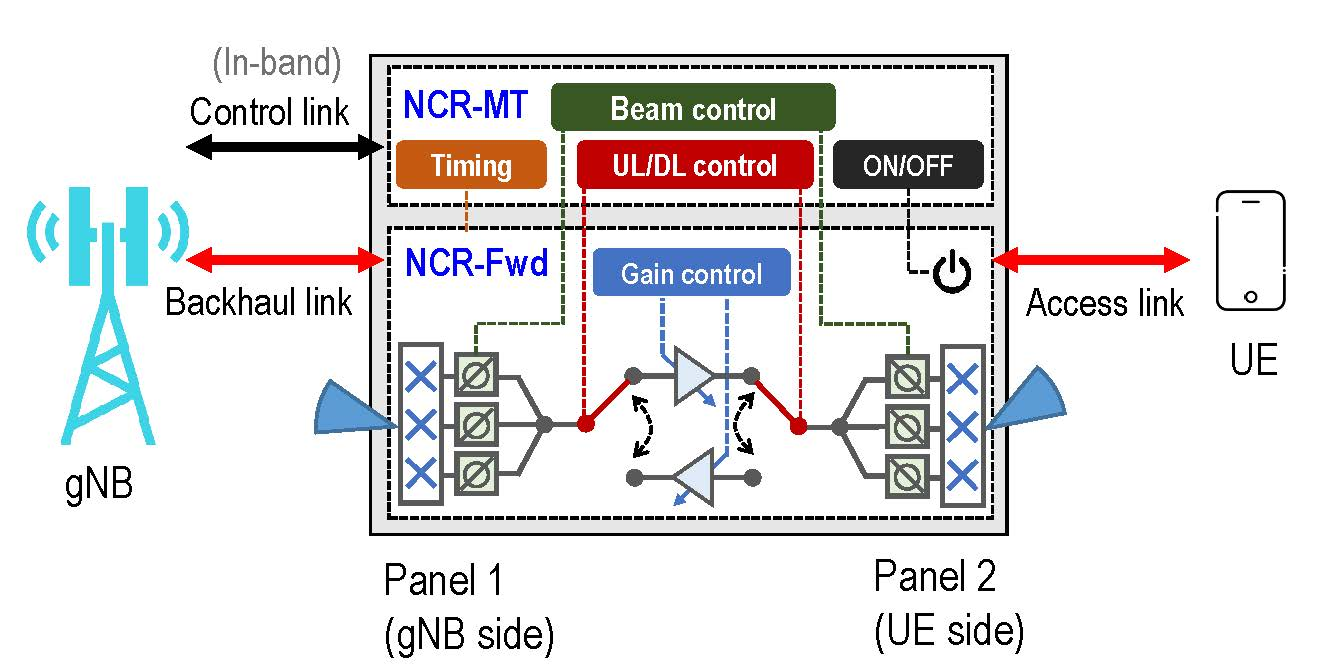
\includegraphics[width=3.5in]{Figs/NCR.jpg}
\caption{NCR architecture.}
\label{fig:NCR}
\end{figure}


As shown in Figure \ref{fig:NCR}, the NCR consists of two functional entities: the NCR-Mobile Termination (NCR-MT) and the NCR-Forwarding (NCR-Fwd), as described in TR38.867 \cite{3GPP-38-867}. The NCR-MT establishes communication with the gNB through a Control link (C-link) using the NR Uu interface. It facilitates the exchange of side control information, such as beamforming, UL/DL switching, and ON/OFF turning, to manage the NCR-Fwd. On the other hand, the NCR-Fwd amplifies and forwards UL/DL RF signals between the gNB and the UE through the backhaul and access links. Its behavior is determined by the side control information received from the gNB.

The NCR-Fwd can be implemented with two sets of panel antennas (one for the backhaul link and the other for the access link) and one RF amplifier (see Figure \ref{fig:NCR}). It amplifies and beamforms the signal before forwarding it in the DL or UL direction. Beamforming techniques allow adjusting the reception and transmission directions. The NCR-Fwd module primarily focuses on signal amplification and (analog) beamforming, eliminating the need for advanced digital receiver or transmitter chains. The performance requirements for beamforming antennas in the NCR-Fwd are not as high as those for macro BS or IAB node antennas. Cost-effectiveness and ease of manufacturing are prioritized.

The NCR-MT and NCR-Fwd can operate in the same or different frequency bands. However, at least one carrier used by the NCR-MT must operate within the frequency band being forwarded by the NCR-Fwd, which serves as the baseline. When the NCR-MT and NCR-Fwd operate in the same frequency band, the C-link and backhaul link will encounter similar large-scale channel properties, simplifying the control of the backhaul link between the gNB and the NCR-Fwd.

The NCR-MT module facilitates the exchange of control and status signaling with the gNB through the C-link, as shown in Figure \ref{fig:NCR}. It is designed to support a subset of UE functions to fulfill its role.

Regarding the transmission and reception of the C-link and backhaul link by the NCR, the following points apply:
\begin{itemize}
\item The DL of the C-link and DL of the backhaul link can be performed simultaneously or in a TDM manner.
\item The UL of the C-link and UL of the backhaul link can be performed in a TDM manner.
\end{itemize}

The gNB controls the multiplexing while considering the capabilities of the NCR. The simultaneous transmission of the UL of the C-link and UL of the backhaul link depends on the NCR's capability.




\subsection{Side Control Information}
TR38.867 \cite{3GPP-38-867} explores various forms of side control information, including but not limited to beam information, ON-OFF information, and TDD DL-UL configuration. The signalling protocol has been designed in detail to accommodate them and summarized in the following subsections.

\subsubsection{Beam Information}

\emph{Backhaul link and C-link}---In the NCR system, both the backhaul link and C-link can utilize fixed or adaptive beamforming techniques.

In the baseline scenario where the NCR-MT and NCR-Fwd operate within the same frequency band, it is expected that the C-link and backhaul link will experience similar large-scale channel characteristics. Therefore, the same transmission configuration indicator (TCI) states used for the C-link can also be applied to the NCR-Fwd for beamforming in the backhaul link.

However, if adaptive beams are employed for both the C-link and backhaul link, the determination and indication of the backhaul link beams can be accomplished through new signaling provided by the gNB. In the absence of indication via the new signaling, the backhaul link beam can be determined based on a predefined rule.


\begin{figure*}
\centering
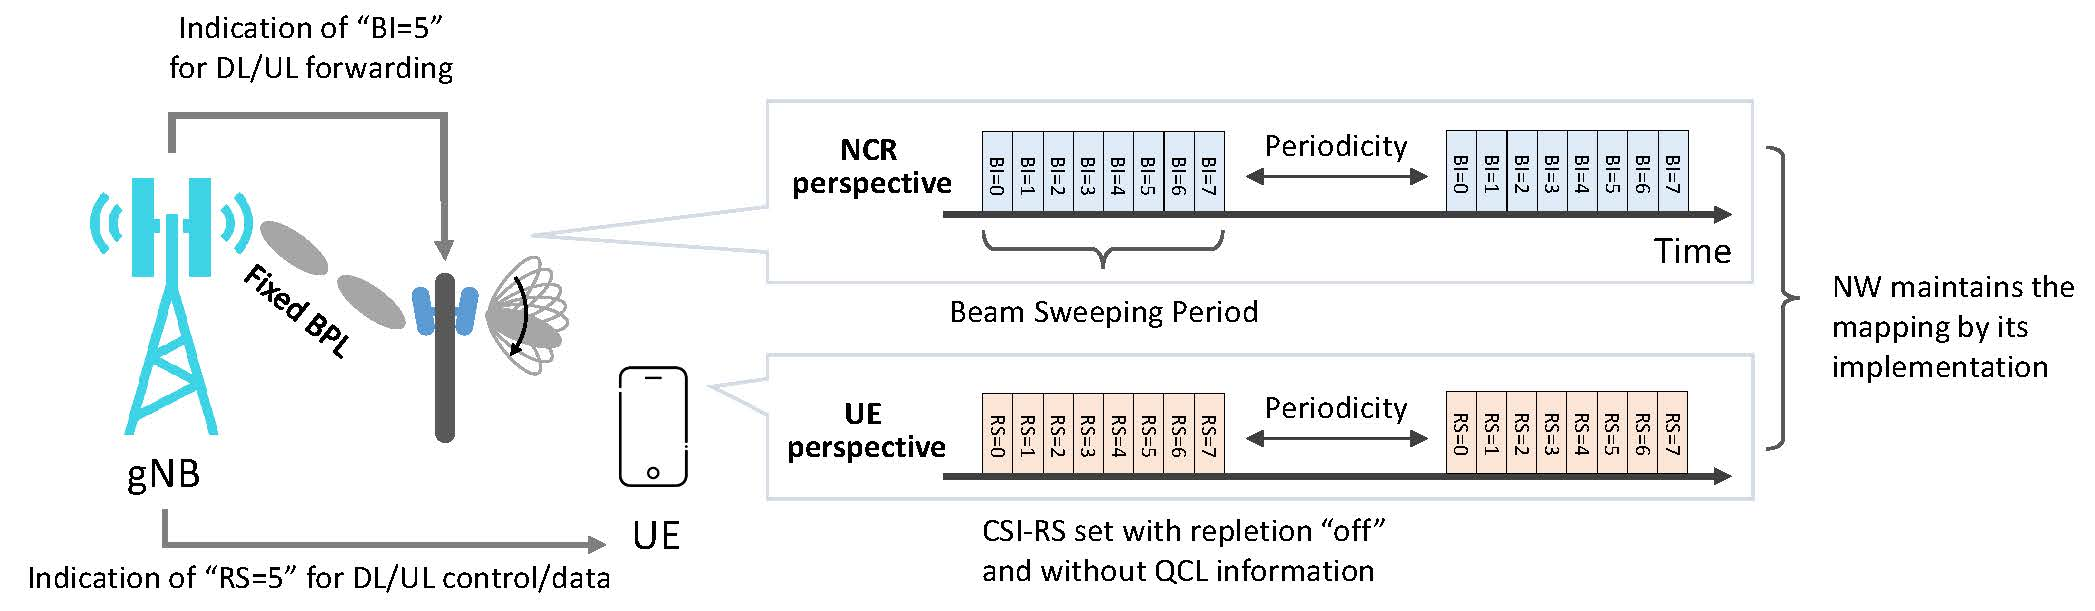
\includegraphics[width=7.0in]{Figs/Beam_Indication.jpg}
\caption{Beam indication for access link.}
\label{fig:Beam_Indication}
\end{figure*}

\emph{Access link}---In the context of the access link, dynamic beam steering towards users, as outlined in TR38.867 \cite{3GPP-38-867}, leads to improved SINR performance compared to fixed-beam solutions, particularly benefiting cell edge users. Additionally, semi-static and dynamic repeater gain/power configurations can further enhance SINR and coverage. These benefits apply to both FR1 and FR2 frequency ranges. Therefore, it is recommended to provide beam information to regulate the behavior of the NCR for the access link.

In NCR-Fwd, the access link beam is indicated using a beam index, considering both dynamic and semi-static indications, including semi-persistent indications. The time domain resource associated with the access link beam is explicitly determined based on the indicated time domain resources. Due to the multiuser scheduling nature, the gNB may frequently change the transmission (Tx) beam of the repeater. This frequent beam switching can result in PDCCH overhead and extended beam-switch delays. As a result, a single beam indication may represent one or multiple beams.

For the DL/UL of the access link in NCR-Fwd, beam correspondence is assumed. The DL and UL beams on the access side that correspond to each other have the same beam index. The forwarding direction of an indicated beam, either DL or UL, is determined based on its corresponding time domain resource and the UL/DL time division duplex (TDD) configuration.

To illustrate the beam indication for the access link, we provide an example depicted in Figure \ref{fig:Beam_Indication}. In this scenario, the gNB guides the NCR through beam control information to perform periodic beam sweeping. The gNB may not have knowledge of the NCR's beam characteristics, while the UE cannot differentiate between beams originating from the gNB or the NCR. Based solely on the received signals, the UE reports its preferred beam index, such as RS=5.

The gNB then indicates Beam Index (BI)=5 as a reference for the NCR's Tx beamforming and designates RS=5 as the QCL type-D RS for determining the Tx beam to the UE. Following the network indication, the NCR can utilize the Tx beam corresponding to RS=5 for subsequent forwarding, starting from a specified application time.

\subsubsection{Timing Information}

As a baseline, the NCR's timing is assumed to follow these guidelines:
\begin{itemize}
\item[-] The NCR-Fwd's DL receive timing aligns with the NCR-MT's DL receive timing.
\item[-] The NCR-Fwd's UL transmit timing aligns with the NCR-MT's UL transmit timing.
\item[-] The NCR-Fwd's DL transmit timing is delayed by an internal delay after the NCR-MT's (or NCR-Fwd's) DL receive timing.
\item[-] The NCR-Fwd's UL receive timing is advanced by an internal delay before the NCR-MT's (or NCR-Fwd's) UL transmit timing.
\end{itemize}

\subsubsection{UL-DL TDD Configuration Information}
For the TDD UL/DL configuration of an NCR, a semi-static TDD UL/DL configuration is supported for the C-link, backhaul link, and access link. The NCR-Fwd has its default behavior set to OFF on the flexible symbols/slots in the semi-static configuration. Additionally, the same TDD UL/DL configuration is assumed to be used for both the backhaul link and access link.

\subsubsection{ON-OFF Information}
Using ON-OFF information allows NCRs to be turned off when not needed, resulting in power savings. TR38.867 \cite{R1-2203237} highlights that ON-OFF information not only saves power but also helps NCRs mitigate interference for high SINR users while maintaining performance for low SINR users, leading to an improved network experience. Therefore, ON-OFF information is recommended for NCRs to control the behavior of NCR-Fwd, providing benefits for network performance. By default, the NCR-Fwd is assumed to be OFF unless explicitly or implicitly indicated by the gNB.


\subsection{Outlook}

Table \ref{tab:IAB_vs_NCR} showcases the narrower scope of NCR in comparison to IAB, primarily due to NCR's early stage of application and specific design objectives. Consequently, enhancements in the side control information for NCR are anticipated. For instance, at the Rel-19 WS, several companies emphasized the necessity of power control to boost NCR performance. Furthermore, strategies such as improvements in beam control and scheduling, and utilizing diverse frequencies for the backhaul link, may also be investigated.

A significant trend observed in Release 18 is the growing transition towards a more UE-centric architecture within the evolution of massive MIMO. One such example is the coherent joint transmission for multi-transmission/reception point (multi-TRP). This shift is motivated by the increasing quantity of UEs, which induces complexities in network management. Consistent with this trend, the concept of a UE-controlled relay or UE-controlled repeater (UCR) has been proposed for potential inclusion in 3GPP Release 19 \cite{RWS-230111}. The UCR employs an amplify-and-forward Layer 1 forwarding with frequency translation (L1 FT-Fwd) mechanism, which relays received signals to the UE using a different frequency band. This method enables end-user-centric collaborative MIMO, as described in \cite{Tsai-TAP22}. Here, multiple fixed or portable devices cooperate to create a rich array of antennas, thereby resulting in substantial performance enhancements.

\section{RIS}

The concept of RIS has yet to be explored by 3GPP. In this section, we review the current status of ETSI Reports, specifically ETSI GR RIS-001 \cite{ETSI-GR-RIS-001} and ETSI GR RIS-003 \cite{ETSI-GR-RIS-003}.

\subsection{Use Cases}

According to ETSI GR RIS-001 \cite{ETSI-GR-RIS-001}, RIS opens a wide range of possibilities. It covers active, passive, and hybrid RIS designs. RIS enables the manipulation of incoming wireless signals using techniques such as reflection, refraction, absorption, backscattering, and various transmission and reception modes. In \cite{ETSI-GR-RIS-001}, RIS is broadly defined as:
\vspace{0.2cm}

\noindent \emph{``RIS is a new type of system node with reconfigurable
surface technology, which can adapt its response according to
the status of the propagation environment through
control signaling.''}

\vspace{0.2cm}

RIS deployment's key use cases include enhancing indoor and outdoor-to-indoor (O2I) coverage, enabling wireless power transfer, facilitating ambient backscattering communications, enhancing positioning accuracy and reliability, and supporting secure communication and privacy protection.


\subsection{Deployment Scenarios}

RIS employs a large number of unit cells to achieve significant performance improvements. Dynamically configuring RIS responses can be challenging, hence understanding the deployment scenarios is crucial for optimizing RIS configurations. Such scenarios include indoor, outdoor, and hybrid environments, with RIS deployed either statically or nomadically.

Network operators and service providers devise control strategies for each scenario. The RIS control plane triggers configurations and obtains real-time states. According to \cite{ETSI-GR-RIS-001}, control plane functions for RIS management can be categorized as follows:
\begin{itemize}
\item \textbf{BS Centralized Management}: RIS is centrally managed by the network through one or more BSs, without coordination between participating BSs.

\item \textbf{BS Distributed Management}: RIS is locally managed by participating BSs, with coordination to avoid conflicts and optimize network performance.

\item \textbf{Autonomous RIS}: RIS optimizes the gain of reflected beams without dedicated control-plane functions, determining optimal configurations based on angular positions.

\item \textbf{UE-controlled RIS}: The UE oversees RIS configuration and operation, providing feedback to the network and deciding on updates based on criteria like data rate and power consumption.
\end{itemize}

\subsection{Requirements}

Although the definition of RIS is broad, \cite{ETSI-GR-RIS-001} suggests several key requirements for RIS:

\begin{itemize}
\item {\bf Hardware Cost}: RIS should be cost-effective compared to relays and repeaters, considering factors such as production, assembly, and component costs, depending on the type of RIS (active, passive, or hybrid).

\item {\bf Ease of Deployment and Maintenance}: RIS deployment should be straightforward, considering fixed or wireless backhaul for control signaling, power supply, and setup complexity. Maintenance should encompass tasks like fault detection, isolation, and software upgrades.

\item {\bf Signal Power Boosting}: The extent of signal power boosting depends on RIS size, the number of elements, and configuration flexibility, providing certain gains comparable to a path without RIS.

\item {\bf Reconfigurability}: Requirements for reconfigurability include timing, resolution, and the extent of configurations, considering timing intervals and the maximum number of simultaneously configurable antenna elements or cells.

\item {\bf Interoperability}: RIS should be interoperable with other wireless systems to enable seamless integration into existing networks.

\item {\bf Regulatory}: RIS should adhere to relevant standards for EM field exposure.
\end{itemize}


\subsection{Communication and Channel Models}

ETSI GR RIS-003 \cite{ETSI-GR-RIS-003} presents the perspective on RIS models for communication, radio localization, and sensing. The report emphasizes the need for channel modeling that strikes a balance between complexity and accuracy, considering factors like frequency ranges, bandwidth, and RIS elements for future studies, including interference analysis and performance evaluation. The channel models prioritize simplicity, considering single RIS reflection and cascaded channels with multiple RIS.

The near-field (Fresnel) and far-field regions exhibit different behaviors for electric and magnetic fields, necessitating distinct path-loss models. The near-field model covers high and low frequency ranges and accommodates various array sizes, making it suitable for short-range and mid-range scenarios.

In addition to channel models, \cite{ETSI-GR-RIS-003} also explores channel estimation, reference scenarios, estimation methods, system designs, and key performance indicators. The methodology facilitates RIS performance evaluation in wireless communications, taking into account the coexistence between network operators and making fair comparisons of transmission techniques, communication protocols, and network deployments.

\subsection{Outlook}

During the Rel-19 WS, various companies and organizations proposed a study or feasibility phase for RIS, advocating for a comprehensive examination of this technology within the 5G Release 19 framework. The shared perspectives among the companies include:
\begin{itemize}
\item \textbf{Channel Modeling}: Several companies proposed to study channel modeling for RIS, including considerations of various propagation phenomena like reflection, refraction, absorption, and scattering. The modeling should account for different scenarios (indoor, outdoor, O2I, LoS/NLoS, etc.), large/small-scale channel variations, radiation patterns, and near/far-field behaviors.

\item \textbf{Use Cases and Deployment Scenarios}: The companies generally proposed to study various use cases, deployment scenarios, and operation modes of RIS, with an emphasis on their potential for improving network coverage and communication performance. This includes investigating RIS's role in both FR1 and FR2 frequency bands and exploring the potential for cooperative transmission and interference mitigation.

\item \textbf{RIS Architecture and Control Signaling}: The companies proposed advanced control information and signaling for RIS, such as power control, signal operation, and beam management, and on the importance of studying how RIS fits into and affects the existing technology architecture. The idea of reusing existing beam management frameworks (such as the one specified in Release 18 NCR) and applying them to RIS was proposed. For instance, a similar architecture of NCR with separated RFs for control and reflection to enhance design flexibility was suggested \cite{Yuan-COMMag22}, as shown in Figure~\ref{fig:RIS}.
\end{itemize}

\begin{figure}
\centering
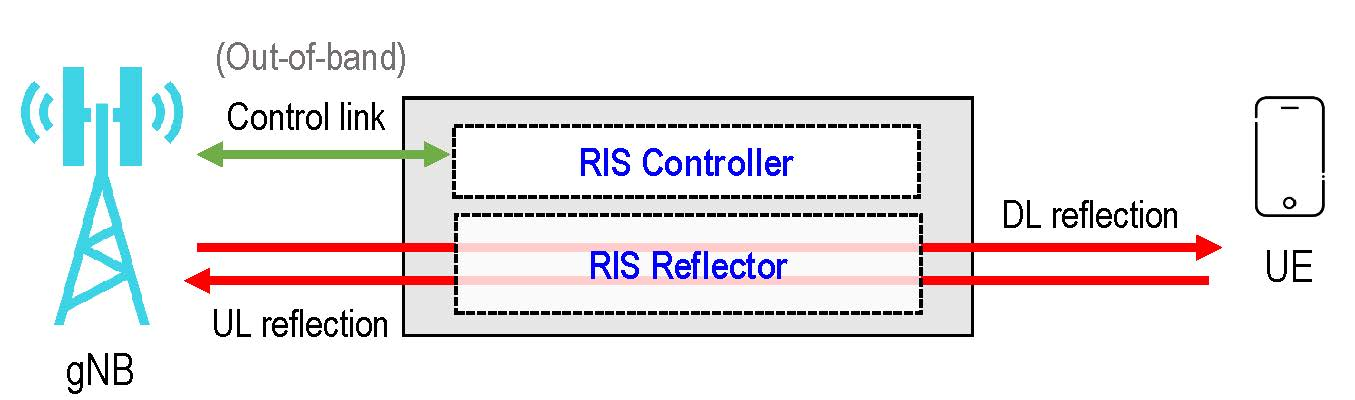
\includegraphics[width=3.5in]{Figs/RIS.jpg}
\caption{Potential RIS architecture. }
\label{fig:RIS}
\end{figure}

\section{Conclusion}

This article provided a comprehensive overview of the 3GPP standardization efforts and deployment considerations of IAB, NCR, and RIS. IAB offers extended coverage and increased capacity through integrated access points, NCR facilitates coverage extension with relays, and RIS enables signal manipulation through reconfigurable unit-cells. These smart electromagnetic entities play a crucial role in the evolution of 5G and its advanced developments, as depicted in Figure \ref{fig:3GPP_Roadmap}. The continued advancements and integration of IAB, NCR, and RIS are expected to significantly shape and enhance the future of wireless communication networks.

{\renewcommand{\baselinestretch}{1.1}
% Generated by IEEEtran.bst, version: 1.14 (2015/08/26)
\begin{thebibliography}{10}
\providecommand{\url}[1]{#1}
\csname url@samestyle\endcsname
\providecommand{\newblock}{\relax}
\providecommand{\bibinfo}[2]{#2}
\providecommand{\BIBentrySTDinterwordspacing}{\spaceskip=0pt\relax}
\providecommand{\BIBentryALTinterwordstretchfactor}{4}
\providecommand{\BIBentryALTinterwordspacing}{\spaceskip=\fontdimen2\font plus
\BIBentryALTinterwordstretchfactor\fontdimen3\font minus
  \fontdimen4\font\relax}
\providecommand{\BIBforeignlanguage}[2]{{%
\expandafter\ifx\csname l@#1\endcsname\relax
\typeout{** WARNING: IEEEtran.bst: No hyphenation pattern has been}%
\typeout{** loaded for the language `#1'. Using the pattern for}%
\typeout{** the default language instead.}%
\else
\language=\csname l@#1\endcsname
\fi
#2}}
\providecommand{\BIBdecl}{\relax}
\BIBdecl

\bibitem{3GPP-Rel10}
\BIBentryALTinterwordspacing
3GPP, ``Overview of {3GPP Release} 10,'' Jul. 2014. [Online]. Available:
  \url{https://www.3gpp.org/ftp/Information/WORK_PLAN/Description_Releases/}
\BIBentrySTDinterwordspacing

\bibitem{TR-23.700}
{3GPP TR 23.700-05}, ``Study on architecture enhancements for vehicle-mounted
  relays {(Release 18)},'' V18.0.0, Dec. 2022.

\bibitem{RP-202813}
RP-202813, ``New {WID} proposal for {NR} repeaters,'' Dec. 2020.

\bibitem{RP-222673}
RP-222673, ``New {WID} on {NR} network-controlled repeaters,'' Sept. 2022.

\bibitem{ETSI-GR-RIS-001}
{ETSI GR RIS}, ``{Reconfigurable Intelligent Surfaces (RIS); Use Cases,
  Deployment Scenarios and Requirements},'' V1.1.1, April 2023.

\bibitem{ETSI-GR-RIS-003}
------, ``{Reconfigurable Intelligent Surfaces (RIS); Communication Models,
  Channel Models, Channel Estimation and Evaluation Methodology},'' V1.1.1,
  June 2023.

\bibitem{Flamini-TAP22}
R.~Flamini \emph{et~al.}, ``Toward a heterogeneous smart electromagnetic
  environment for millimeter-wave communications: An industrial viewpoint,''
  \emph{IEEE Trans. on Ant. and Prop.}, vol.~70, no.~10, pp. 8898--8910, 2022.

\bibitem{TS-38.300}
{3GPP TS 38.300}, ``{NR and NG-RAN Overall description, Stage-2},'' V16.4.0,
  Release 16, Jan. 2021.

\bibitem{IAB-Overview22}
\BIBentryALTinterwordspacing
V.~F.~Monteiro \emph{et~al.}, ``Paving the way towards mobile {IAB}: Problems,
  solutions and challenges,'' 2022. [Online]. Available:
  \url{https://arxiv.org/abs/2206.14946}
\BIBentrySTDinterwordspacing

\bibitem{IAB-chae}
G.-Y. Suk \emph{et~al.}, ``Full-duplex integrated access and backhaul for {5G
  NR}: Analyses and prototype measurements,'' \emph{IEEE Wireless Comm.},
  vol.~29, no.~4, pp. 40--46, 2022.

\bibitem{3GPP-38-867}
{3GPP TR 38.867}, ``Study on {NR} network-controlled repeaters,'' Oct. 2022.

\bibitem{R1-2203237}
R1-2203237, ``Discussion on side control information to enable {NR}
  network-controlled,'' ZTE, May 2022.

\bibitem{RWS-230111}
RWS-230111, ``Device collaborative {Tx} and {Rx},'' MediaTek Inc., RAN-Release
  19 Workshop, Taipei, June 2023.

\bibitem{Tsai-TAP22}
\BIBentryALTinterwordspacing
{L.-S. Tsai, S.-L. Shih, P.-K. Liao, and C.-K. Wen}, ``{MIMO} evolution toward
  {6G}: End-user-centric collaborative {MIMO},'' May 2023. [Online]. Available:
  \url{https://arxiv.org/abs/2305.12308}
\BIBentrySTDinterwordspacing

\bibitem{Yuan-COMMag22}
Y.~Yuan, D.~Wu, Y.~Huang, and C.-L. I, ``Reconfigurable intelligent surface
  relay: Lessons of the past and strategies for its success,'' \emph{IEEE Comm.
  Mag.}, vol.~60, no.~12, pp. 117--123, 2022.

\end{thebibliography}




\end{document}


